\documentclass{exercise}

\institute{Lehr- und Forschungsgebiet Kontinuumsmechanik}
\title{Übung 8}
\author{Joshua Feld, 406718}
\course{Mechanik verformbarer Körper}
\professor{Itskov}
\semester{Sommersemester 2022}
\program{CES (Bachelor)}

\begin{document}
    \maketitle


    \section*{Aufgabe 1}

    \begin{problem}
        Gegeben sind die in der Abbildung gezeigten Träger.
        Die Kantenlänge eines Gitterelements sei als \(a\) bekannt.
        \begin{enumerate}
            \item Berechnen Sie Flächenträgheitsmomente \(I_y\) und \(I_z\).
            \item Welche Erkenntnis lässt sich aus den Ergebnissen ableiten.
        \end{enumerate}
        \begin{center}
            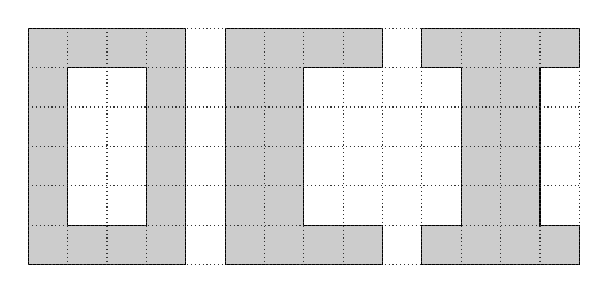
\begin{tikzpicture}[scale=.5]
                \draw[fill=white!80!black] (0,0) rectangle (4,-6);
                \draw[fill=white] (1,-1) rectangle (3,-5);
                \draw[fill=white!80!black] (5,0) -- (9,0) -- (9,-1) -- (7,-1) -- (7,-5) -- (9,-5) -- (9,-6) -- (5,-6) -- cycle;
                \draw[fill=white!80!black] (10,0) -- (14,0) -- (14,-1) -- (13,-1) -- (13,-5) -- (14,-5) -- (14,-6) -- (10,-6) -- (10,-5) -- (11,-5) -- (11,-1) -- (10,-1) -- cycle;
                \foreach \i in {0,1,...,14}
                {
                    \draw[densely dotted,white!20!black] (\i,0) -- (\i,-6);
                }
                \foreach \i in {0,-1,...,-6}
                {
                    \draw[densely dotted,white!20!black] (0,\i) -- (14,\i);
                }
            \end{tikzpicture}
        \end{center}
    \end{problem}

    \subsection*{Lösung}
    \begin{enumerate}
        \item\,
        \begin{center}
            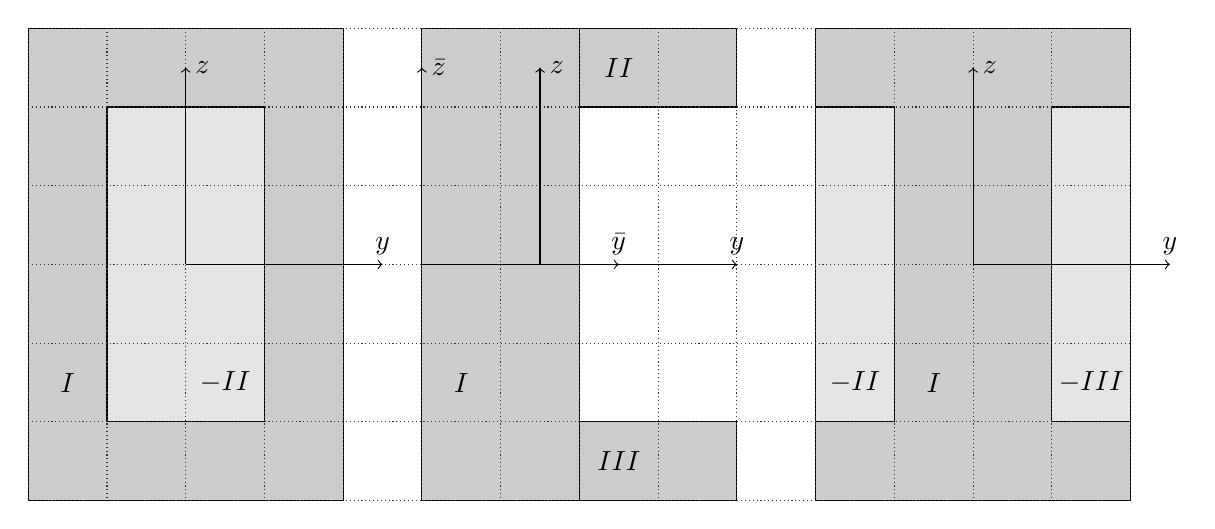
\begin{tikzpicture}
                \draw[fill=white!80!black] (0,0) rectangle (4,-6);
                \draw[fill=white!90!black] (1,-1) rectangle (3,-5);
                \draw[fill=white!80!black] (5,0) -- (9,0) -- (9,-1) -- (7,-1) -- (7,-5) -- (9,-5) -- (9,-6) -- (5,-6) -- cycle;
                \draw (7,0) -- (7,-6);
                \draw[fill=white!80!black] (10,0) rectangle (14,-6);
                \draw[fill=white!90!black] (10,-1) rectangle (11,-5);
                \draw[fill=white!90!black] (13,-1) rectangle (14,-5);
                \foreach \i in {0,1,...,14}
                {
                    \draw[densely dotted,white!20!black] (\i,0) -- (\i,-6);
                }
                \foreach \i in {0,-1,...,-6}
                {
                    \draw[densely dotted,white!20!black] (0,\i) -- (14,\i);
                }
                \node at (0.5,-4.5) {\(I\)};
                \node at (2.5,-4.5) {\(-II\)};
                \draw[->] (2,-3) -- (2,-.5) node[right] {\(z\)};
                \draw[->] (2,-3) -- (4.5,-3) node[above] {\(y\)};
                \node at (5.5,-4.5) {\(I\)};
                \node at (7.5,-.5) {\(II\)};
                \node at (7.5,-5.5) {\(III\)};
                \draw[->] (5,-3) -- (5,-.5) node[right] {\(\bar{z}\)};
                \draw[->] (5,-3) -- (7.5,-3) node[above] {\(\bar{y}\)};
                \draw[->] (6.5,-3) -- (6.5,-.5) node[right] {\(z\)};
                \draw[->] (6.5,-3) -- (9,-3) node[above] {\(y\)};
                \node at (11.5,-4.5) {\(I\)};
                \node at (10.5,-4.5) {\(-II\)};
                \node at (13.5,-4.5) {\(-III\)};
                \draw[->] (12,-3) -- (12,-.5) node[right] {\(z\)};
                \draw[->] (12,-3) -- (14.5,-3) node[above] {\(y\)};
            \end{tikzpicture}
        \end{center}
        \begin{enumerate}
            \item Der Schwerpunkt ist in der Mitte des Trägers.
            Wir können unser Koordinatensystem direkt in den Schwerpunkt legen.
            Teilen wir die Geometrie in ein (positives) äußeres Rechteck \(I\) und ein (negatives) inneres Rechteck \(II\) auf ergibt sich sofort
            \begin{align*}
                I_{y, l} &= I_{y, I} - I_{y, II} = 72a^4 - \frac{32}{3}a^4 = \frac{184}{3}a^4,\\
                I_{z, l} &= I_{z, I} - I_{z, II} = 32a^4 - \frac{8}{3}a^4 = \frac{88}{3}a^4,
            \end{align*}
            wobei keine Steiner-Anteile berechnet werden müssen, da der Schwerpunkt beider Teilgeometrien im Ursprung des gewählten Koordinatensystems liegt.
            \item Der Schwerpunkt ist nicht direkt erkennbar und muss zuerst ermittelt werden.
            Hierzu werden drei Teilbereiche \(I\), \(II\) und \(III\) gebildet.
            Ausgehend vom \(\bar{y}\)-\(\bar{z}\)-Koordinatensystem ergibt sich:
            \begin{center}
                \begin{tabular}{lccccc}
                    \toprule
                    \(i\) & \(A_i\) & \(\bar{y}_{s, i}\) & \(\bar{y}_{s, i}A_i\) & \(\bar{z}_{s, i}\) & \(\bar{z}_{s, i}A_i\)\\
                    \midrule
                    \(I\) & \(12a^2\) & \(a\) & \(12a^3\) & \(0\) & \(0\)\\
                    \(II\) & \(2a^2\) & \(3a\) & \(6a^3\) & \(\frac{5}{2}a\) & \(5a^3\)\\
                    \(III\) & \(2a^2\) & \(3a\) & \(6a^3\) & \(-\frac{5}{2}a\) & \(-5a^3\)\\
                    \midrule
                    \(\sum\) & \(16a^2\) & & \(24a^3\) & & \(0\)\\
                    \bottomrule
                \end{tabular}
            \end{center}
            \[
                \bar{y}_s = \frac{1}{A}\sum y_{s, i}A_i = \frac{24a^3}{16^2} = \frac{3}{2}a, \quad \bar{z}_s = \frac{1}{A}\sum z_{s, i}A_i = 0.
            \]
            Für die Flächenträgheitsmomente folgt
            \begin{center}
                \begin{tabular}{lccccc}
                    \toprule
                    \(i\) & \(A_i\) & \(I_{y, i}\) & \(\bar{z}_{s, i}\) & \(\bar{z}_s\) & \(\parentheses*{\bar{z}_{s, i} - \bar{z}_s}^2 A_i\)\\
                    \midrule
                    \(I\) & \(12a^2\) & \(36a^4\) & \(0\) & \(0\) & \(0\)\\
                    \(II\) & \(2a^2\) & \(\frac{1}{6}a^4\) & \(\frac{5}{2}a\) & \(0\) & \(\frac{25}{2}a^4\)\\
                    \(III\) & \(2a^2\) & \(\frac{1}{6}a^4\) & \(-\frac{5}{2}a\) & \(0\) & \(\frac{25}{2}a^4\)\\
                    \midrule
                    \(\sum\) & \(16a^2\) & \(\frac{109}{3}a^4\) & & & \(25a^4\)\\
                    \bottomrule
                \end{tabular}
            \end{center}
            \[
                I_{y, m} = \sum I_{y, i} + \sum\parentheses*{\bar{z}_{s, i} - \bar{z}_s}^2 A_i = \frac{109}{3}a^4 + 25a^4 = \frac{184}{3}a^4,
            \]
            \begin{center}
                \begin{tabular}{lccccc}
                    \toprule
                    \(i\) & \(A_i\) & \(I_{z, i}\) & \(\bar{y}_{s, i}\) & \(\bar{y}_s\) & \(\parentheses*{\bar{y}_{s, i} - \bar{y}_s}^2 A_i\)\\
                    \midrule
                    \(I\) & \(12a^2\) & \(4a^4\) & \(a\) & \(\frac{3}{2}a\) & \(3a^4\)\\
                    \(II\) & \(2a^2\) & \(\frac{2}{3}a^4\) & \(3a\) & \(\frac{3}{2}a\) & \(\frac{9}{2}a^4\)\\
                    \(III\) & \(2a^2\) & \(\frac{2}{3}a^4\) & \(3a\) & \(\frac{3}{2}a\) & \(\frac{9}{2}a^4\)\\
                    \midrule
                    \(\sum\) & \(16a^2\) & \(\frac{16}{3}a^4\) & & & \(12a^4\)\\
                    \bottomrule
                \end{tabular}
            \end{center}
            \[
                I_{z, m} = \sum I_{z, i} + \sum\parentheses*{\bar{y}_{s, i} - \bar{y}_s}^2 A_i = \frac{16}{3}a^4 + 12a^4 = \frac{52}{3}a^4.
            \]
            Hierbei war es nötig Steiner-Anteile zu berücksichtigen, da die Einzelteile nicht im Ursprung des gewählten Koordinatensystems lagen.
            \item Der Schwerpunkt ist in der Mitte des Trägers.
            Wir können unser Koordinatensystem direkt in den Schwerpunkt legen.
            Teilen wir die Geometrie in ein (positives) äußeres Rechteck \(I\) und zwei (negative) seitliche Rechtecke \(II\) und \(III\) ergibt sich für die Flächenträgheitsmomente
            \begin{center}
                \begin{tabular}{lccccc}
                    \toprule
                    \(i\) & \(A_i\) & \(I_{y, i}\) & \(\bar{z}_{s, i}\) & \(\bar{z}_s\) & \(\parentheses*{\bar{z}_{s, i} - \bar{z}_s}^2 A_i\)\\
                    \midrule
                    \(I\) & \(24a^2\) & \(72a^4\) & \(0\) & \(0\) & \(0\)\\
                    \(-II\) & \(\parentheses*{-}4a^2\) & \(\parentheses*{-}\frac{16}{3}a^4\) & \(0\) & \(0\) & \(0\)\\
                    \(-III\) & \(\parentheses*{-}4a^2\) & \(\parentheses*{-}\frac{16}{3}a^4\) & \(0\) & \(0\) & \(0\)\\
                    \midrule
                    \(\sum\) & \(16a^2\) & \(\frac{184}{3}a^4\) & & & \(0\)\\
                    \bottomrule
                \end{tabular}
            \end{center}
            \[
                I_{y, r} = \sum I_{y, i} + \sum\parentheses*{\bar{z}_{s, i} - \bar{z}_s}^2 A_i = \frac{184}{3}a^4,
            \]
            \begin{center}
                \begin{tabular}{lccccc}
                    \toprule
                    \(i\) & \(A_i\) & \(I_{z, i}\) & \(\bar{y}_{s, i}\) & \(\bar{y}_s\) & \(\parentheses*{\bar{y}_{s, i} - \bar{y}_s}^2 A_i\)\\
                    \midrule
                    \(I\) & \(24a^2\) & \(32a^4\) & \(0\) & \(0\) & \(0\)\\
                    \(-II\) & \(\parentheses*{-}4a^2\) & \(\parentheses*{-}\frac{1}{3}a^4\) & \(-\frac{3}{2}a\) & \(0\) & \(\parentheses*{-}9a^4\)\\
                    \(-III\) & \(\parentheses*{-}4a^2\) & \(\parentheses*{-}\frac{1}{3}a^4\) & \(\frac{3}{2}a\) & \(0\) & \(\parentheses*{-}9a^4\)\\
                    \midrule
                    \(\sum\) & \(16a^2\) & \(\frac{94}{3}a^4\) & & & \(-18a^4\)\\
                    \bottomrule
                \end{tabular}
            \end{center}
            \[
                I_{z, r} = \sum I_{z, i} + \sum\parentheses*{\bar{y}_{s, i} - \bar{y}_s}^2 A_i = \frac{94}{3}a^4 - 18a^4 = \frac{40}{3}a^4.
            \]
            Hierbei war es nötig Steiner-Anteile zu berücksichtigen, da die Einzelteile nicht im Ursprung des gewählten Koordinatensystems lagen.
            Es ist zu beachten, dass beim Aufsummieren der Flächen, Trägheitsmomente und Steiner-Anteile die Flächen, die abgezogen werden, mit einem negativen Vorzeichen eingehen.
        \end{enumerate}
        \item Es ist zu sehen, dass \(A\) und \(I_y\) für alle Trägertypen gleich sind, während \(I_z\) variiert.
        Folgendes lässt sich daraus erkennen:
        \begin{itemize}
            \item Alle Träger verbrauchen exakt gleich viel Material und sind daher gleich schwer.
            \item Bei Biegung um die \(y\)-Achse sind alle Träger gleich stabil.
            \item Bei Biegung um die \(z\)-Achse ist der linke Träger am stabilsten und der rechte Träger am schwächsten.
        \end{itemize}
    \end{enumerate}


    \section*{Aufgabe 2}

    \begin{problem}
        Für den im Bild dargestellten unsymmetrischen Querschnitt sind zu berechnen:
        \begin{enumerate}
            \item die Flächenträgheitsmomente \(I_y\) und \(I_z\) und das Deviationsmoment \(I_{yz}\) bezüglich der Schwerpunktachsen,
            \item die Hauptträgheitsmomente \(I_1\) und \(I_2\),
            \item die Lage der Hauptachsen.
        \end{enumerate}
        \begin{center}
            \begin{tikzpicture}[scale=.75]
                \draw (0,0) -- (5,0) -- (5,-.75) -- (2,-.75) -- (2,-7) -- (1.25,-7) -- (1.25,-1) -- (0,-1) -- cycle;
                \draw[|<->|] (-.25,0) -- (-.25,-1) node[midway,left] {\(20\)};
                \draw[|<->|] (0,.25) -- (1.25,.25) node[midway,above] {\(25\)};
                \draw[<->|] (1.25,.25) -- (2,.25) node[midway,above] {\(15\)};
                \draw[<->|] (2,.25) -- (5,.25) node[midway,above] {\(60\)};
                \draw[|<->|] (5.25,0) -- (5.25,-.75) node[midway,right] {\(15\)};
                \draw[<->|] (5.25,-.75) -- (5.25,-7) node[midway,right] {\(125\)};
                \fill (1.9,-2.5) circle (1mm) node[above right] {\(S\)};
                \draw[dashed,->] (2.9,-2.5) -- (.9, -2.5) node[below] {\(y\)};
                \draw[dashed,->] (1.9,-1.5) -- (1.9,-3.5) node[right] {\(z\)};
            \end{tikzpicture}
        \end{center}
    \end{problem}

    \subsection*{Lösung}
    \begin{enumerate}
        \item Der Schwerpunkt ist nicht direkt erkennbar und muss zuerst ermittelt werden.
        Hierzu werden drei Teilbereiche \(I\) (großes Rechteck rechts, \(75 \times 140\)), \(II\) (negatives Rechteck unten rechts, \(60 \times 125\)) und \(III\) (kleines Rechteck oben links, \(20 \times 25\)) gebildet.
        Ausgehend von einem Koordinatensystem in der oberen linken Ecke ergibt sich:
        \begin{center}
            \begin{tabular}{lccccc}
                \toprule
                \(i\) & \(A_i\) & \(\bar{y}_{s, i}\) & \(\bar{y}_{s, i}A_i\) & \(\bar{z}_{s, i}\) & \(\bar{z}_{s, i}A_i\)\\
                \midrule
                \(I\) & \(10500\) & \(-62,5\) & \(-656250\) & \(70\) & \(735000\)\\
                \(-II\) & \(\parentheses*{-}7500\) & \(-70\) & \(\parentheses*{-}-525000\) & \(77,5\) & \(\parentheses*{-}581250\)\\
                \(III\) & \(500\) & \(-12,5\) & \(-6250\) & \(10\) & \(5000\)\\
                \midrule
                \(\sum\) & \(3500\) & & \(-137500\) & & \(158750\)\\
                \bottomrule
            \end{tabular}
        \end{center}
        \begin{align*}
            \bar{y}_s &= \frac{1}{A}\sum y_{s, i}A_i = -\frac{137500}{3500} = -\frac{275}{7} = -39,29\sis{\milli\meter},\\
            \bar{z}_s &= \frac{1}{A}\sum z_{s, i}A_i = \frac{158750}{3500} = \frac{635}{14} = 45,36\sis{\milli\meter}.
        \end{align*}
        Mit den Abkürzungen \(\Delta z_{s, i} = \bar{z}_{s, i} - \bar{z}_s\) und \(\Delta y_{s, i} = \bar{y}_{s, i} - \bar{y}_s\) folgt für die Flächenträgheitsmomente
        \begin{center}
            \begin{tabular}{lcccc}
                \toprule
                \(i\) & \(A_i\) & \(I_{y, i}\) & \(\Delta z_{s, i}\) & \(\Delta z_{s, i}^2 A_i\)\\
                \midrule
                \(I\) & \(10500\) & \(17,15 \cdot 10^6\) & \(24,64\) & \(6,375 \cdot 10^6\)\\
                \(-II\) & \(\parentheses*{-}7500\) & \(\parentheses*{-}9,757 \cdot 10^6\) & \(32,14\) & \(\parentheses*{-}7,747 \cdot 10^6\)\\
                \(III\) & \(500\) & \(0,017 \cdot 10^6\) & \(-35,36\) & \(0,625 \cdot 10^6\)\\
                \midrule
                \(\sum\) & \(3500\) & \(7,41 \cdot 10^6\) & & \(-0,747 \cdot 10^6\)\\
                \bottomrule
            \end{tabular}
        \end{center}
        \[
            I_y = \sum I_{y, i} + \sum\parentheses*{\bar{z}_{s, i} - \bar{z}_s}^2 A_i = 7,41 \cdot 10^6 - 0,747 \cdot 10^6 = 6,663 \cdot 10^6\sis{\milli\meter\tothe{4}},
        \]
        \begin{center}
            \begin{tabular}{lcccc}
                \toprule
                \(i\) & \(A_i\) & \(I_{z, i}\) & \(\Delta y_{s, i}\) & \(\Delta y_{s, i}^2 A_i\)\\
                \midrule
                \(I\) & \(10500\) & \(4,922 \cdot 10^6\) & \(-23,21\) & \(5,656 \cdot 10^6\)\\
                \(-II\) & \(\parentheses*{-}7500\) & \(\parentheses*{-}2,25 \cdot 10^6\) & \(-30,71\) & \(\parentheses*{-}7,073 \cdot 10^6\)\\
                \(III\) & \(500\) & \(0,026 \cdot 10^6\) & \(26,79\) & \(0,359 \cdot 10^6\)\\
                \midrule
                \(\sum\) & \(3500\) & \(2,698 \cdot 10^6\) & & \(-1,058 \cdot 10^6\)\\
                \bottomrule
            \end{tabular}
        \end{center}
        \[
            I_z = \sum I_{z, i} + \sum\parentheses*{\bar{y}_{s, i} - \bar{y}_s}^2 A_i = 2,698 \cdot 10^6 - 1,058 \cdot 10^6 = 1,64 \cdot 10^6\sis{\milli\meter\tothe{4}},
        \]
        \begin{center}
            \begin{tabular}{lccccc}
                \toprule
                \(i\) & \(A_i\) & \(I_{yz, i}\) & \(\Delta y_{s, i}\) & \(\Delta z_{s, i}\) & \(\Delta y_{s, i}\Delta z_{s, i} A_i\)\\
                \midrule
                \(I\) & \(10500\) & \(0\) & \(-23,21\) & \(24,64\) & \(-6,005 \cdot 10^6\)\\
                \(-II\) & \(\parentheses*{-}7500\) & \(0\) & \(-30,71\) & \(32,14\) & \(\parentheses*{-}-7,403 \cdot 10^6\)\\
                \(III\) & \(500\) & \(0\) & \(26,79\) & \(-35,36\) & \(-0,474 \cdot 10^6\)\\
                \midrule
                \(\sum\) & \(3500\) & \(0\) & & & \(0,924 \cdot 10^6\)\\
                \bottomrule
            \end{tabular}
        \end{center}
        \[
            I_{yz} = \sum I_{yz, i} + \sum\parentheses*{\bar{y}_{s, i} - \bar{y}_s}\parentheses*{\bar{z}_{s, i} - \bar{z}_s} A_i = -0,924 \cdot 10^6\sis{\milli\meter\tothe{4}}.
        \]
        \item Mit der Formel für die Hauptträgheitsmomente gilt
        \[
            I_{1, 2} = \frac{I_y + I_z}{2} \pm \sqrt{\parentheses*{\frac{I_y - I_z}{2}}^2 + I_{yz}^2}
        \]
        und somit
        \[
            I_1 = 6,819 \cdot 10^6\sis{\milli\meter\tothe{4}}, \quad I_2 = 1,475 \cdot 10^6\sis{\milli\meter\tothe{4}}.
        \]
        \item Aus der Gleichung für den Winkel
        \[
            \tan\parentheses*{2\varphi^*} = \frac{2I_{yz}}{I_y - I_z}
        \]
        folgt
        \[
            \varphi^* = -10,125^\circ.
        \]
        Das Einsetzen in die Transformationsgleichungen liefert die korrekte Zuordnung der beiden Hauptachsenwinkel zu den Hauptträgheitsmomenten
        \[
            \varphi_1^* = \varphi^* = -10,125^\circ, \quad \varphi_2^* = \varphi^* + 90^\circ = 79,875^\circ.
        \]
    \end{enumerate}


    \section*{Aufgabe 3}

    \begin{problem}
        Von einem Rechteck mit gegebenen Seitenlängen soll ein Dreieck so abgeschnitten werden, dass beim Aufhängen des entstehenden Trapezes in \(A\) die Grundlinie parallel zur \(\bar{y}\)-Achse liegt.
        \begin{enumerate}
            \item Wie lang muss die Strecke \(c\) gewählt werden?
            \item Berechnen Sie für das entstehende Trapez die Lage des Flächenschwerpunktes, die Flächenträgheitsmomente, das Deviationsmoment, die Hauptträgheitsmomente sowie die Lage der Hauptträgheitsachsen.
        \end{enumerate}
        \begin{center}
            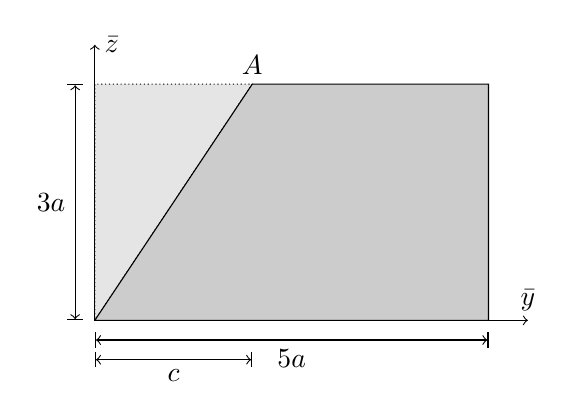
\begin{tikzpicture}
                \draw[densely dotted,fill=white!90!black] (0,0) -- (2,3) -- (0,3) -- cycle;
                \draw[fill=white!80!black] (0,0) -- (2,3) node[above] {\(A\)} -- (5,3) -- (5,0) -- cycle;
                \draw[->] (0,0) -- (5.5,0) node[above] {\(\bar{y}\)};
                \draw[->] (0,0) -- (0,3.5) node[right] {\(\bar{z}\)};
                \draw[|<->|] (-.25,0) -- (-.25,3) node[midway,left] {\(3a\)};
                \draw[|<->|] (0,-.25) -- (5,-.25) node[midway,below] {\(5a\)};
                \draw[|<->|] (0,-.5) -- (2,-.5) node[midway,below] {\(c\)};
            \end{tikzpicture}
        \end{center}
        Gegeben: \(a\)
    \end{problem}

    \subsection*{Lösung}
    \begin{enumerate}
        \item In dieser Aufgabe soll nach dem Entfernen des Dreiecks ein Aufhängen im Punkt \(A\) stattfinden.
        Dabei soll die Grundfläche des Trapezes wie bisher parallel zur \(\bar{y}\)-Achse verlaufen.
        Umformuliert bedeutet dies, dass der Schwerpunkt exakt unter \(A\) liegen muss, damit sich die Struktur nicht dreht.
        Im gegebenen Koordinatensystem entspricht dies der Bedingung \(\bar{y}_s = c\).

        Für den Schwerpunkt ergibt sich in Abhängigkeit von \(a\) und \(c\)
        \begin{center}
            \begin{tabular}{lccccc}
                \toprule
                \(i\) & \(A_i\) & \(\bar{y}_{s, i}\) & \(\bar{y}_{s, i}A_i\) & \(\bar{z}_{s, i}\) & \(\bar{z}_{s, i}A_i\)\\
                \midrule
                \(I\) & \(15a^2\) & \(-62,5\) & \(-656250\) & \(70\) & \(735000\)\\
                \(-II\) & \(\parentheses*{-}\frac{3}{2}ac\) & \(\frac{1}{3}c\) & \(\parentheses*{-}\frac{1}{2}ac^2\) & \(2a\) & \(\parentheses*{-}3a^2 c\)\\
                \midrule
                \(\sum\) & \(3a\parentheses*{5a - \frac{1}{2}c}\) & & \(\frac{1}{2}a\parentheses*{75a^2 - c^2}\) & & \(\frac{3}{2}a^2\parentheses*{15a - 6c}\)\\
                \bottomrule
            \end{tabular}
        \end{center}
        \begin{align*}
            \bar{y}_s &= \frac{1}{A}\sum y_{s, i}A_i = \frac{\frac{1}{2}a\parentheses*{75a^2 - c^2}}{3a\parentheses*{5a - \frac{1}{2}c}} = \frac{75a^2 - c^2}{3 \cdot \parentheses*{10a - c}},\\
            \bar{z}_s &= \frac{1}{A}\sum z_{s, i}A_i = \frac{\frac{3}{2}a^2\parentheses*{15a - 6c}}{3a\parentheses*{5a - \frac{1}{2}c}} = \frac{a\parentheses*{15a - 2c}}{10a - c}.
        \end{align*}
        Mit der Bedingung \(\bar{y}_s = c\) folgt durch Umformen die quadratische Gleichung
        \[
            c^2 - 15ac + \frac{75}{2}a^2 = 0
        \]
        mit den beiden Lösungen
        \[
            c_{1, 2} = \frac{15}{2}a \pm \sqrt{\frac{225}{4}a^2 - \frac{75}{2}a^2} = \frac{15}{2}a \pm \frac{5\sqrt{3}}{2}a,
        \]
        wobei die Lösung \(c_2 = \frac{15 + 5\sqrt{3}}{2}a\) größer als die Breite des Rechtecks ist und daher entfällt.
        Es gilt somit
        \[
            c = c_1 = \frac{15 - 5\sqrt{3}}{2}a = 3,17a.
        \]
        \item Es gilt
        \[
            \bar{y}_s = \frac{75a^2 - c^2}{3 \cdot \parentheses*{10a - c}} = 3,17a, \quad \bar{z}_s = \frac{a\parentheses*{15a - 2c}}{10a - c} = 1,27a.
        \]
        Mit den Abkürzungen \(\Delta z_{s, i} = \bar{z}_{s, i} - \bar{z}_s\) und \(\Delta y_{s, i} = \bar{y}_{s, i} - \bar{y}_s\) folgt für die Flächenträgheitsmomente
        \begin{center}
            \begin{tabular}{lcccc}
                \toprule
                \(i\) & \(A_i\) & \(I_{y, i}\) & \(\Delta z_{s, i}\) & \(\Delta z_{s, i}^2 A_i\)\\
                \midrule
                \(I\) & \(15a^2\) & \(\frac{45a^4}{4}\) & \(0,23a\) & \(0,794a^4\)\\
                \(-II\) & \(\parentheses*{-}\frac{3}{2}ac\) & \(\parentheses*{-}\frac{3ca^3}{4}\) & \(0,73a\) & \(\parentheses*{-}2,534a^4\)\\
                \midrule
                \(\sum\) & \(3a\parentheses*{5a - \frac{1}{2}c}\) & \(\frac{a^3\parentheses*{45a - 3c}}{4}\) & & \(-1,74a^4\)\\
                \bottomrule
            \end{tabular}
        \end{center}
        \[
            I_y = \sum I_{y, i} + \sum\parentheses*{\bar{z}_{s, i} - \bar{z}_s}^2 A_i = 7,133a^4,
        \]
        \begin{center}
            \begin{tabular}{lcccc}
                \toprule
                \(i\) & \(A_i\) & \(I_{z, i}\) & \(\Delta y_{s, i}\) & \(\Delta y_{s, i}^2 A_i\)\\
                \midrule
                \(I\) & \(15a^2\) & \(\frac{125a^4}{4}\) & \(-0,67a\) & \(6,734a^4\)\\
                \(-II\) & \(\parentheses*{-}\frac{3}{2}ac\) & \(\parentheses*{-}\frac{ac^3}{12}\) & \(-2,11a\) & \(\parentheses*{-}21,17a^4\)\\
                \midrule
                \(\sum\) & \(3a\parentheses*{5a - \frac{1}{2}c}\) & \(\frac{a\parentheses*{375a^3 - c^3}}{12}\) & & \(-14,436a^4\)\\
                \bottomrule
            \end{tabular}
        \end{center}
        \[
            I_z = \sum I_{z, i} + \sum\parentheses*{\bar{y}_{s, i} - \bar{y}_s}^2 A_i = 14,159a^4,
        \]
        \begin{center}
            \begin{tabular}{lccccc}
                \toprule
                \(i\) & \(A_i\) & \(I_{yz, i}\) & \(\Delta y_{s, i}\) & \(\Delta z_{s, i}\) & \(\Delta y_{s, i}\Delta z_{s, i} A_i\)\\
                \midrule
                \(I\) & \(15a^2\) & \(0\) & \(-0,67a\) & \(0,23a\) & \(-2,312a^4\)\\
                \(-II\) & \(\parentheses*{-}\frac{3}{2}ac\) & \(\parentheses*{-}-1,256a^4\) & \(-2,11a\) & \(0,73a\) & \(\parentheses*{-}-7,324a^4\)\\
                \midrule
                \(\sum\) & \(3a\parentheses*{5a - \frac{1}{2}c}\) & \(1,256a^4\) & & & \(5,012a^4\)\\
                \bottomrule
            \end{tabular}
        \end{center}
        \[
            I_{yz} = \sum I_{yz, i} + \sum\parentheses*{\bar{y}_{s, i} - \bar{y}_s}\parentheses*{\bar{z}_{s, i} - \bar{z}_s} A_i = -3,756a^4.
        \]
        Für die Hauptflächenträgkeitsmomente ergibt sich
        \[
            I_{1, 2} = \frac{I_y + I_z}{2} \pm \sqrt{\parentheses*{\frac{I_y - I_z}{2}}^2 + I_{yz}^2}
        \]
        \[
            I_1 = 15,733a^4, \quad I_2 = 5,492a^4.
        \]
        Der Winkel zwischen der \(y\)-Achse und einer Hauptachse ergibt sich aus
        \[
            \tan\parentheses*{2\varphi^*} = \frac{2I_{yz}}{I_y - I_z} \implies \varphi^* = 23,457^\circ.
        \]
        Aus den Transformationsgleichungen folgt, dass es sich hierbei um \(\varphi_2^*\) handelt.
    \end{enumerate}
\end{document}
